\documentclass[a4paper, 12pt, titlepage]{article}
\usepackage{amssymb,amsthm,amsmath} %ams
\usepackage[finnish]{babel} %suomenkielinen tavutus
\usepackage[fixlanguage]{babelbib}
\selectbiblanguage{finnish}
\usepackage[T1]{fontenc} %skanditavutus
\usepackage[utf8x]{inputenc}        	% skandit utf-8 koodauksella
%\usepackage[ansinew]{inputenc}        	% skandit utf-8 koodauksella, kokeile tata, jos utf-8 ylla ei toimi.
\usepackage{graphicx}
%\usepackage{qtree}% yksinkertaiset puut
\usepackage{tikz}% vähän tehokkaampi grafiikkapaketti
\usepackage{url}
\usepackage[nottoc]{tocbibind}% viitteet sisällysluetteloon
\usepackage[linesnumbered, boxed]{algorithm2e}
\usepackage{subcaption} % for side by side figures
\usepackage[hang,flushmargin]{footmisc}
%\usepackage{cite}
\usepackage[square]{natbib}% käytetään nyt natbibiä eikä citeä
\setcitestyle{notesep={}}% kun laitetaan \citep[.]{lähde}, niin lähteen ja . väliin ei tule ", "

\let\oldnl\nl %vanha komento \nl talteen \oldnl
\newcommand{\nonl}{\renewcommand{\nl}{\let\nl\oldnl}} %poista rivinumero yhdeltä riviltä
%suomennoksia yo. paketille:
\renewcommand*{\algorithmcfname}{Algoritmi}
\renewcommand*{\listalgorithmcfname}{Lista algoritmeista}
%ja sisällysluettelolle
\addto\captionsfinnish{
 \renewcommand{\contentsname}{Sisällys}}

\linespread{1.24} %1.24 olisi rivivali 1.5
\sloppy % Vahentaa tavutuksen tarvetta, "leventamalla" rivin keskella olevia valilyönteja.

% Yleisimmin kayttettaville komennoille voi maaritella lyhynnemerkintöja
% esimerkiksi
\newcommand{\R}{\mathbb{R}}
\newcommand{\abs}[1]{\vert #1 \vert} % Itseisarvo
\newcommand{\tab}[1][0.5cm]{\hspace*{#1}} % Sisennys
\newcommand{\code}[1]{\small\texttt{#1}} % Monospace-fontti koodille

\setlength\parindent{0pt} %uuden kappaleen sisennys

\addtolength{\leftmargin}{4cm}
\addtolength{\rightmargin}{3cm}

\title{Avaruusjakoon perustuvat tietorakenteet tietokonegrafiikassa}
\author{Timo Heinonen \\kandidaatintutkielma \\ tietojenkäsittelytiede \\ Turun yliopisto}
\date{Lokakuu 2016}
%\pagestyle{headings} 

\begin{document}

\begin{titlepage}
 %\begin{figure}
 %
\includegraphics[width=3cm]{img/soihtu.png}
 %\vspace{4.0cm}
 %\end{figure}

 \vspace*{5.0cm}

 \begin{center}\Large
  Avaruusjakoon perustuvat tietorakenteet tietokonegrafiikassa
 \end{center}

\vfill

 \begin{raggedleft}
  TURUN YLIOPISTO\\
  Informaatioteknologian laitos\\
  tietojenkäsittelytieteet\\
  \today\\
  kandidaatintutkielma\\
  Timo Heinonen\\
 \end{raggedleft}

 \begin{figure}[b]
  \makebox[\textwidth]{
\includegraphics[width=\paperwidth]{img/footer.png}}
  \vspace*{-5.0cm}
 \end{figure}
\end{titlepage}


\newpage
\pagenumbering{gobble}% Ei sivunumeroita
\thispagestyle{empty}
\section*{Tiivistelmä}
\setlength{\hoffset}{-1in} \setlength{\oddsidemargin}{4cm} \addtolength{\textwidth}{1.3cm} \addtolength{\textheight}{1cm} \setlength{\voffset}{-1in}
\thispagestyle{empty}  %ei sivunumeroa sivun alareunaan

\noindent
TURUN YLIOPISTO\\
Informaatioteknologian laitos\\
\\
HEINONEN, TIMO: Avaruusjakoon perustuvat tietorakenteet tietokonegrafiikassa\\
kandidaatintutkielma, \pageref{LastPage} s.\\
Tietojenkäsittelytieteet\\
\today\\
\rule{\textwidth}{.2mm}\\
\\
Tässä tutkielmassa tutustutaan kolmiulotteisten kuvien hahmontamiseen kaksiulotteisiksi kuviksi säteenseurannaksi kutsutulla tekniikalla. Säteenseurannalla saadaan muodostettua realistisia kuvia, mutta se on laskennollisesti erittäin raskasta. Tästä syystä hahmonnuksen kohteena olevasta maisemasta muodostetaan ennen hahmonnusta avaruuden osiin jakamiseen perustuva tietorakenne, jota läpikäymällä voidaan vähentää tarvittavien laskutoimitusten määrää.

\vspace{4mm}

Avaruusjakorakenteista esitetään BSP-puu, sen erikoistapaus kd-puu ja rajaavien tilojen hierarkia BVH. Oikein muodostettuna näitä rakenteita käyttämällä voidaan vähentää hahmontamisessa tarvittavia säteiden ja monikulmioiden leikkausta testaavia operaatioita logaritmiseen määrään verrattuna niin sanottuun brute force -toteutukseen. 

\vspace{4mm}

Lopuksi vertaillaan tietorakenteita keskenään ja yritetään löytää niistä sellainen, joka nopeuttaisi säteenseurantaa eniten. Tulokset hahmontamisen nopeudessa vaihtelevat kuitenkin kuvattavien maisemien, käytettyjen implementaatioiden sekä laitteistojen välillä niin paljon, ettei parasta tietorakennetta pystytä osoittamaan.

%\vspace{4mm}

\vfill
\vspace{4mm}Asiasanat: tietokonegrafiikka, säteenseuranta, avaruusjako, BSP-puu, kd-puu, rajaava tila, BVH.


\newpage
\pagenumbering{arabic}% Sivunumerot takaisin

%\setcounter{tocdepth}{2} % Sisennys ToC:iin
\tableofcontents


\newpage
\section{Johdanto}

Kolmiulotteisen tietokonegrafiikkan tutkimuksella on ollut merkittävä vaikutus viihdeteollisuuteen, kuten animaatioelokuviin, peleihin ja virtuaalitodellisuuteen, sekä tietokoneavusteiseen suunnitteluun, esimerkiksi arkktehtuurin ja teollisuuden alalla. \citep{wald04}  Tietokonegrafiikka on osin jopa syrjäyttämässä perinteistä valokuvaustyötä: huonekalujätti Ikea on siirtynyt käyttämään myyntikuvastoissaan valtaosin tietokoneella generoituja kuvia valokuvien sijaan \citep{ikea}. Tietokonegrafiikan sovelluskohteet lisääntyvät jatkuvasti. Eräs aktiivinen tutkimuskohde on esimerkiksi tietokonegrafiikan tekniikoiden soveltaminen konenäköön. \citep[.]{hughes}\\

Grafiikan piirtämistä kolmiulotteisista malleista kaksiulotteisiksi kuviksi kutsutaan hahmontamiseksi (engl. \emph{rendering}). Hahmontamisen lähtökohtana on kuvattava maisema (engl. \emph{scene}), joka sisältää objekteja ja valonlähteitä. Objektit ja valonlähteet on voitava mallintaa matemaattisesti, jotta niille voidaan määrittää sijainti ja suuntaus ja jotta niiden välisiä etäisyyksiä ja suhteita voidaan laskea. Hahmontaminen tapahtuu aina jostakin kuvakulmasta, ja tätä varten määritellään virtuaalinen kamera, jolla on oma sijaintinsa ja suuntauksensa maisemassa. Tämän jälkeen on selvitettävä, mitkä objektit kamera näkee, miten objekteihin osuvat valonsäteet vaikuttavat niiden väriin ja kuvan varjostukseen. Lopuksi lasketaan mitkä värit projisoidaan kuvatason mihinkin pikseliin. \citep[.]{janke}\\

1960-luvulla tietokonegrafiikkaa käytettiin lähinnä teollisuuden komponenttisuunnittelussa ja arkkitehtuurissa. Tietokoneella osattiin piirtää objektien ääriviivoja (engl. \emph{wireframe}), mutta varjostustekniikoita ei tunnettu. IBM:n tutkija Arthur Appel esitteli algoritmin, joka mallinsi valonsäteitä laskemalla suoran yhtälöitä kuvasta maisemaan ja siitä valonlähteisiin. Tämän tekniikan avulla voitiin piirtää yksinkertaisia varjostuksia. \citep[.]{appel}. Myöhemmin tästä säteenseurannaksi nimetystä tekniikasta tuli erittäin suosittu.\\

Jo Appel totesi säteenseurannan olevan erittäin laskennallisesti raskasta \citep{appel}. Vaikka tietokoneiden ja varsinkin grafiikkaprosessoreiden laskentateho kasvaa jatkuvasti, ei grafiikan tuottaminen ole vieläkään halpaa tai nopeaa. Kuvista halutaan jatkuvasti realistisempia, ja yksityiskohtaisemmat kuvattavat mallit ja monimutkaiset valaisutekniikat vaativat erittäin paljon laskentatehoa. Esimerkiksi elokuvastudio Pixarin Monsterit-yliopisto -animaatioelokuvan piirtäminen vaati yli sata miljoonaa prosessorituntia \citep{monsterit}. Tämän takia tutkimuksen kohteena on ollut jo pitkään entistä nopeampien hahmontamistekniikoiden kehittäminen.\\
%Prosessoritunti?

1980-luvulla kehitettiin menetelmiä, joilla voitiin nopeuttaa hahmontamista vähentämällä valonsäteiden ja maiseman osumatarkasteluiden määrää. Steven Rubin ja Turner Whitted esittelivät tekniikan, jossa maisema ositetaan esiprosessointivaiheessa manuaalisesti hierarkisiin laatikoihin. Säteiden ja laatikoiden osumia tarkastelemalla voitiin vähentää operaatioiden kokonaismäärää. \citep[.]{rubin} Henry Fuchs et al. kehittivät toisen metodin, johon kuului myös esiprosessointivaihe, tällä kertaa tietokoneen suorittamana. Maiseman objektit oli jaettu pienempiin monikulmioihin, joista valittiin binääripuun juureksi mahdollisimman keskellä maisemaa oleva.\\
%oleva?

Tässä tutkielmassa esitellään avaruuden jakamiseen perustuvia tietorakenteita, joilla kolmiulotteisten kuvien hahmontamista voidaan nopeuttaa. Luvussa 2 määritellään joitakin grafiikan peruskäsitteitä sekä esitetään algoritmi säteenseurannalle. Luvussa 3 tutkitaan binääristä avaruusjakoa, kd-puuta ja rajaavien tilojen hierarkiaa sekä niiden rakentamiseen ja läpikäyntiin liittyviä algoritmeja. Luvussa 4 vertaillaan edellä mainittuja tietorakenteita ja niiden soveltuvuutta säteenseuranta-algoritmin optimoimiseen.

%Historiaa kakkoslukuun?

\newpage
\section{Kolmiulotteisen tietokonegrafiikan peruskäsitteitä}
\subsection{Määritelmiä}

Kolmiulotteisten kuvien hahmontamisen kohteena ovat \emph{objektit}, jotka mallintavat jotakin esinettä tai muotoa avaruudessa $\R^3$. Objektit voidaan esittää tietokoneen muistissa taulukkona pisteitä $P=(x,y,z)\;\epsilon\,\R^3$: esimerkiksi kolmiota voidaan kuvata kolmella pisteellä ja palloa kahdella pisteellä, jotka esittävät sen keskipistettä ja yhtä pistettä sen pinnalla. \citep[.]{angel}\\

Objektit jaetaan lähes kaikissa ei-triviaaleissa tapauksissa monikulmioihin (engl. \emph{polygoneihin}). Monikulmio $\gamma = \diamond P_1P_2...P_n, \; n > 2$, on samassa tasossa olevien kärkien $P_1,...,P_n$ muodostaman murtoviivan rajaama alue, jonka kärkien muodostamat janat $P_i P_{i+1}$ eivät leikkaa toisiaan muualla kuin kärjissä \citep{harju}. Useimmiten grafiikkasovelluksissa ja -rajapinnoissa valitaan monikulmioiden kärkien lukumääräksi kolmi, sillä kolmioiden kärjet muodostavat aina tason, ja grafiikkaprosessorit osaavat operoida kolmioilla erittäin nopeasti \citep{angel}.\\

Objektien sisäpuoli halutaan yleensä jättää huomioimatta, joten monikulmioille on määriteltävä, kummalla puolella on niiden etupuoli. Kolmiot ovat tässäkin suhteessa hyvä valinta monikulmioiden muodoksi, sillä kolmiolle $\triangle P_1P_2P_3$ voidaan helposti laskea etupuolen määrittävä normaali $n$ ristitulolla $(P_2-P_1) \times (P_3-P_2)$. Huomioitavaa on, että normaalin suunta riippuu siitä, missä järjestyksessä kärjet $P_1, P_2$ ja $P_3$ on määritelty. \citep[.]{hughes}\\

Jotta voitaisiin tarkastella objektien, valonlähteiden, ja kuvakulman eli \emph{kameran} välisiä suhteita ja suuntauksia avaruudessa, valitaan kolme koordinaatistoa, jotka on määritelty kolmella toisiinsa nähden kohtisuoralla kantavektorilla $(\vec{i},\vec{j},\vec{k})$. Jokaisella objektilla on \emph{lokaalikoordinaatisto}, joka sisältää objektin geometrian. Useimmiten origo sijoitetaan objektin keskipisteeseen. \emph{Maailmakoordinaatisto} kuvaa koko avaruutta ja sisältää tietoa siitä, mihin objektien lokaalikoordinaatistojen origot on sijoitettu. Lopuksi tämä maisema kuvataan virtuaalisella kameralla, jolla on oma \emph{kamerakoordinaatistonsa}. Koordinaatistosta toiseen siirtyminen, koordinaatistojen skaalaus ja rotaatio voidaan toteuttaa lineaarikuvauksilla. \citep[.]{janke}

\subsection{Säteenseuranta}

\emph{Säteenseuranta} (engl. \emph{Ray Tracing}) on hahmontamistekniikka, jolla voidaan piirtää erittäin fotorealistisia kuvia. Säteenseuranta pyrkii mallintamaan valonsäteitä, jotka saavat alkunsa valonlähteistä, kulkevat avaruudessa ja osuvat objekteihin, jolloin ne valaisevat niitä, kimpoavat niistä toisiin objekteihin ja muodostavat varjoja. Jotkut valonsäteet löytävät lopulta tiensä katsojan silmiin eli kameraan. Koska olisi mahdotonta selvittää jokaisen valonsäteen kulkua avaruudessa, säteenseuranta-algoritmi ottaa huomioon vain ne säteet, jotka todella osuvat kameraan. Valonsäteitä seurataan siis käänteisessä järjestyksessä, kamerasta objekteihin, ja niistä valonlähteisiin. Säteenseurantatekniikkaa on havainnollistettu kuvassa \ref{raytracing}. \citep[.]{janke}\\

Säteenseuranta-algoritmi muodostaa sille syötteenä annetusta kolmiulotteisesta maisemasta kameran sijainnin perusteella kaksiulotteisen kuvan. Jokaisen kuvatason pikselin läpi ammutaan säde $\vec{R}=O+t\vec{D}$, missä $t\,\epsilon\,\R$, $O$ on kameran sijainti maailmakoordinaatistossa ja normalisoitu vektori $\vec{D}$ kuvaa säteen kulkusuuntaa. Säteellä etsitään törmäyspistettä lähimmän objektin kanssa eli sellaista mahdollisimman pientä arvoa $t$, että piste $P=O+t\vec{D}$ on jonkin objektin pinnalla. Tällöin osuman saaneen objektin piste $P$ voi näkyä kameraan, mikäli siihen osuu valoa.\footnote{Tämä on niin kutsuttu \emph{näkyvyysongelma}.} Osumakohdasta ammutaan uusi, varjostussäteeksi kutsuttu säde. Jos varjostussäde osuu suoraan tai kimmoten muista objekteista valonlähteeseen, lankeaa objektin pinnalle valoa.\footnote{Tässä tutkielmassa huomiomatta varjostus, joka on oleellinen osa hahmontamista. Hyvä lähtöpiste realistiseen varjostukseen ja valaistukseen tutustumiseen on esimerkiksi James Kajiyan hahmontamisyhtälö \citep[ks.][]{kajiya}.}  \citep[.]{janke} Jos monikulmioiden muodoksi on valittu kolmiot, voidaan säteen ja kolmion leikkaus määrittää esimerkiksi nopealla Möllerin-Trumboren algoritmilla \citep[ks.][]{moller}. Säteenseurantatekniikan pseudokoodi on esitetty algoritmissa \ref{algo_raytrace}.\\


%Järjestys tässä?
Algoritmin suoritusnopeutta rajoittaa se, että jokaista sädettä kohti on käytävä läpi kaikki maiseman monikulmiot ja testattava, osuuko säde niihin. Säteiden ja monikulmioiden leikkauksien määrittämiseen joudutaan joissain tapauksissa käyttämään jopa 95 \% koko laskenta-ajasta \citep{whitted}. Algoritmia saataisiin siis nopeutettua huomattavasti, jos testattavien monikulmioiden määrää jokaista sädettä kohti saataisiin vähennettyä. Yleisesti käytetty tapa leikkaustestien vähentämiseksi on muodostaa maisemasta hierarkinen tietorakenne ennen varsinaista hahmontamista. Tätä tietorakennetta läpikäymällä löydetään nopeasti monikulmio, jonka pinnalla säteen ja objektin leikkauspiste $P$ on. \citep[.]{rubin}\\

Säteenseurantaa on perinteisesti sen hitauden vuoksi hyödynnetty hahmontamisessa, jossa käytetty laskenta-aika saakin venyä pitkäksi. Peleissä, virtuaalitodellisuudessa ja muissa reaaliaikaista hahmontamista vaativissa sovelluksissa on käytetty pitkälti niink utsuttua kolmioiden rasterointitekniikkaa (engl. \emph{rasterization}). Säteenseurannalla hahmonnetut kuvat ovat kuitenkin huomattavasti realistisempia kuin rasteroinnilla saavutetut, joten reaaliaikainen hahmontaminen Säteenseurantatekniikalla on suosittu tutkimuskohde. \citep[.]{wald04}  
 

\begin{figure}
 \centering 
 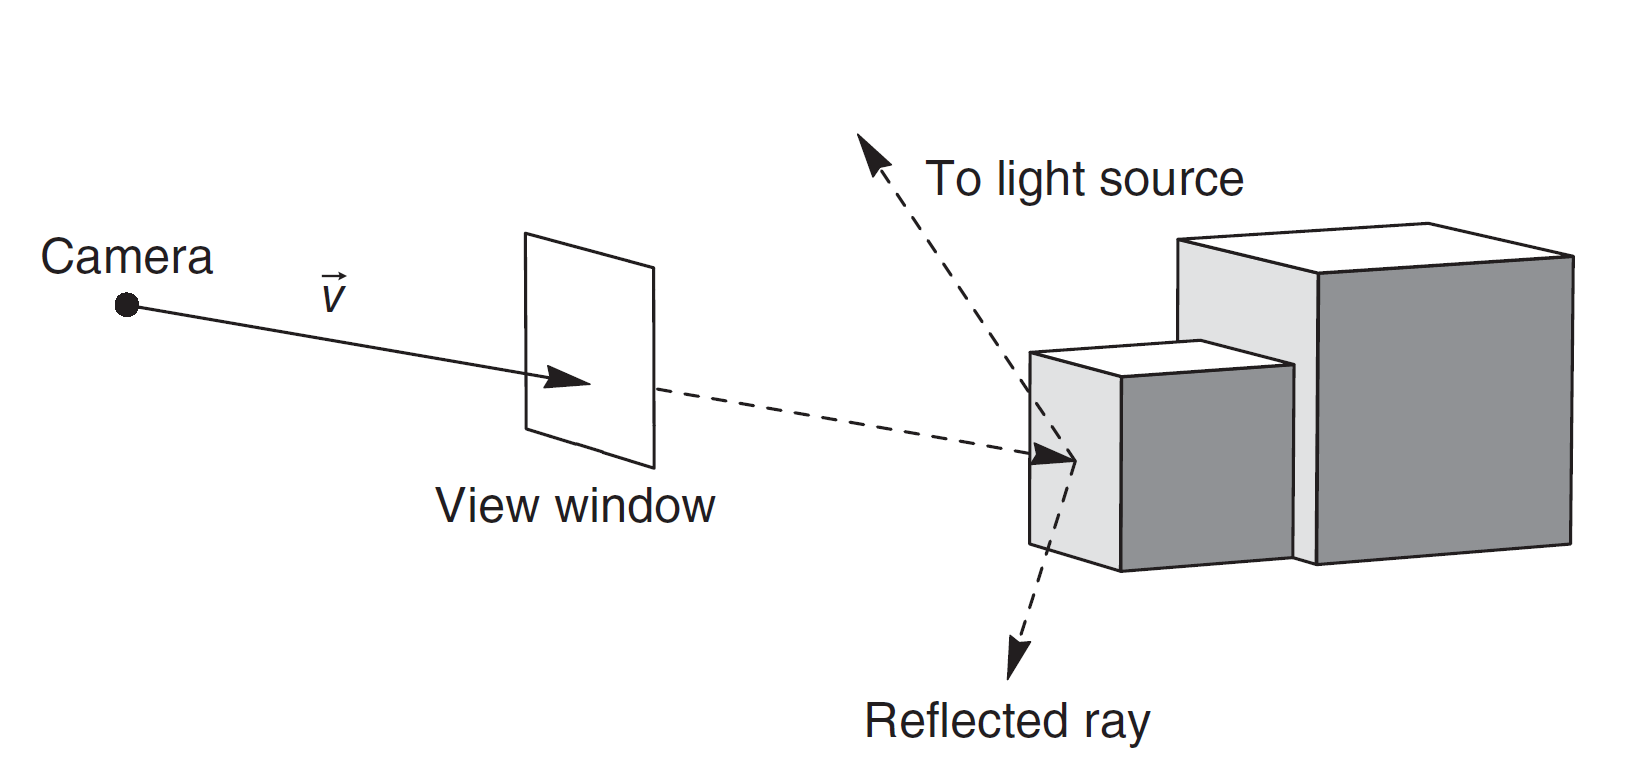
\includegraphics[width=0.9\textwidth]{img/raytracing.png}
 \vspace{0.4cm}
 \caption{Säteen ampuminen kuvan läpi maisemaan \citep{janke}}
 \label{raytracing}
 \vspace{-0.5cm}
\end{figure}

\begin{algorithm}[htp]
\small
\KwIn{\\\texttt{kuvataso}: $x*y$ kokoinen taulukko pikseleitä \\
\texttt{maisema}: joukko valonlähteitä ja monikulmioihin jaettuja objekteja}
\KwOut{\\kolmiulotteinen maisema projisoituna \texttt{kuvataso}lle}
\BlankLine
\nonl \texttt{RAY\_TRACING(kuvataso, maisema)}:\\
\ForEach{pikseli $(x,y) \; \epsilon$ \textnormal{\texttt{kuvataso}}}{
  \texttt{etaisyys} $\gets \infty$ \\
  \ForEach{monikulmio $\epsilon$ \textnormal{\texttt{maisema}}}{
    Ammu säde $\vec{R}=O+t\vec{D}$ kamerasta pikselin läpi \textnormal{\texttt{maisema}}an \\
    \eIf{säde $\vec{R}$ osui monikulmioon pisteessä $P$ {\bf and} t < \textnormal{\texttt{etaisyys}}}{
	\texttt{etaisyys} $\gets t$\\ 
      	Valon määrä $V \gets 0$\\
	\ForEach{valonlähde $L$}{
	Ammu varjostussäde $\vec{R_s}=L-P$ valonlähdettä kohti\\
	Kasvata valosummaa $V$               
      }
      Aseta pikselin $(x,y)$ väri valosumman $V$ mukaisesti
    }{
      Aseta pikseli $(x,y)$ taustan väriseksi
    }
  }
}
\KwRet \texttt{kuvataso}
\caption{\texttt{RAY\_TRACING}}
\label{algo_raytrace}
\end{algorithm}

\vspace{-0.5cm}

\newpage
\section{Avaruusjakopuut}

Tässä luvussa esitellään kaksi tekniikkaa avaruuden ositukseen säteenseurannan nopeuttamiseksi. Binääriseksi avaruusjaoksi kutsutaan tekniikkaa, jossa avaruutta jaetaan rekursiivisesti kahteen pienempään osaan. Binääriseen avaruusjakoon liittyvistä tietorakenteista esitellään BSP-puu ja sen erikoistapaus kd-puu. Toinen keino jakaa maisemaa nopeammin käsiteltäviin osiin on hahmotella objekteja ryhmiin ja muodostaa jokaiselle objektille niin kutsuttu rajaava tila. Tällä tekniikalla voidaan muodostaa puun muotoinen rajavien tilojen hierarkia. 

\subsection{Binäärinen avaruusjako}
\subsubsection{BSP-puu}

Eräs suosittu avaruusjakoon perustuva tietorakenne on binäärinen avaruusjakopuu, eli \emph{BSP-puu} (engl. \emph{Binary Space Partitioning}). BSP-puu luodaan valitsemalla kolmiulotteisen maiseman  monikulmiojoukosta $\Gamma$ yksi monikulmio $\gamma_k$, joka asetetaan puun juureksi. monikulmion $\gamma_k$ muodostama taso jakaa maiseman, ja siten monikulmiojoukon $\Gamma$, kahteen osaan $\Gamma_{k,+}$ ja $\Gamma_{k,-}$. Joukko $\Gamma_{k,+}$ sisältää monikulmion $\gamma_k$ positiivisella puolella olevat monikulmiot, ja siten ne asetetaan BSP-puuhun juuren oikeaksi lapseksi. Vastaavasti joukko $\Gamma_{k,-}$ sisältää negatiivisella puolella olevat monikulmiot, ja kuuluvat monikulmion $\gamma_k$ vasemmaksi lapseksi. Tämä jakavan monikulmion valinta ja avaruuden jako niin sanotuiksi \emph{vokseleiksi} (engl. \emph{voxel, volume element}) suoritetaan rekursiivisesti BSP-puun lehdille, kunnes jokaisessa lehdessä on vain yksi tai ennaltamäärätty määrä monikulmioita. \citep[.]{samet} BSP-puun rakentamisen pseudokoodi on esitelty algoritmissa \ref{algo_bsp}.\\

BSP-puuta ja sen solmuja voidaan esittää grafiikkasovelluksessa seuraavasti:\\\\%\citep{ranta}
\code{
class BSP\_Tree\\
\{\\
\tab BSP\_Node juuri\\
\}\\\\
class BSP\_Node\\
\{\\
\tab Polygon jakaja\\
\tab BSP\_Node* oikea\_lapsi\\
\tab BSP\_Node* vasen\_lapsi\\
\tab Polygon monikulmiot[$\,$] \tab //joukko monikulmioita, josta alipuut\\ 
\hspace*{5.2cm} //muodostetaan\\
\}\\}

\begin{algorithm}[htp]
\small
\KwIn{\\
\texttt{BSP\_Node solmu}:\hspace{1.54cm} juurisolmu, josta puu rakennetaan\\
\texttt{Polygon monikulmiot[$\,$]}: monikulmiojoukko, josta alipuut rakennetaan}
\KwOut{\\BSP-puu, jonka juurena on solmu \texttt{node}}
\BlankLine
\nonl \texttt{RAKENNA\_BSP\_PUU(solmu, monikulmiot):\\}
 \texttt{jakaja} $\gets$ \texttt{VALITSE\_JAKAVA\_MONIKULMIO(monikulmiot)}\\
 \texttt{positiivinen\_joukko} $\gets \emptyset$\\
 \texttt{negatiivinen\_joukko} $\gets \emptyset$\\
 \ForEach{\textnormal{\texttt{$\gamma \, \epsilon$ monikulmiot}}}{
   \texttt{sijainti} $\gets$ \texttt{VERTAA($\gamma$, jakaja)}\\
  \uIf{\textnormal{\texttt{sijainti} = jakajan edessä}}{
   \texttt{positiivinen\_joukko} = \texttt{positiivinen\_joukko} $\cup\;\gamma$
  }
  \uElseIf{\textnormal{\texttt{sijainti} = jakajan takana}}{
   \texttt{negatiivinen\_joukko} = \texttt{negatiivinen\_joukko} $\cup\;\gamma$
  }
  \ElseIf{\textnormal{\texttt{sijainti} = leikkaa jakajan määrittämää tasoa}}{
   \texttt{JAA\_MONIKULMIO($\gamma$, jakaja, $\Gamma_{jakaja,+}$, $\Gamma_{jakaja,-}$)}\\
   \texttt{positiivinen\_joukko} = \texttt{positiivinen\_joukko} $\cup\;\Gamma_{jakaja,+}$\\
   \texttt{negatiivinen\_joukko} = \texttt{negatiivinen\_joukko} $\cup\;\Gamma_{jakaja,-}$
  }  
 }
\If{\textnormal{\texttt{positiivinen\_joukko}} $\neq \emptyset$}{
 \texttt{RAKENNA\_BSP\_PUU(solmu.oikea\_lapsi, positiivinen\_joukko)}
}
\If{\textnormal{\texttt{positiivinen\_joukko}} $\neq \emptyset$}{
 \texttt{RAKENNA\_BSP\_PUU(solmu.vasen\_lapsi, negatiivinen\_joukko)}
}

\caption{\texttt{RAKENNA\_BSP\_PUU \citep{ranta}}}\label{algo_bsp}
\end{algorithm}


\vspace{-0.5cm}

Kuvissa \ref{bsp1}-\ref{bsp2} on esitetty esimerkki BSP-puun muodostamisesta. Kuvassa \ref{bsp11} on yksinkertaisuuden vuoksi esitetty monikulmiot $\Gamma=\{A,B,C,D,E,F,G\}$ sisältävä maisema kaksiulotteisena. Kuvassa \ref{bsp12} ensimmäiseksi jakomonikulmioksi on valittu $G$, jonka positiiviselle puolelle jäävät monikulmiot $\Gamma_{g,+} = \{A,B,C\}$, ja negatiiviselle puolelle $\Gamma_{g,-} = \{D,E,F\}$. Jaon g negatiivinen puoli saadaan jaettua loppuun asti ongelmitta valitsemalla jakomonikulmioksi $E$, mutta jos positiivisella puolella valitaan jakomonikulmioksi $B$, joudutaan monikulmio $C$ jakamaan osiin $C_1$ ja $C_2$. Jakolinjan $b$ negatiiviselle puolelle jää vain yksi monikulmio $C_2$, joten jaettavaksi jää vain $b$:n positiivinen puoli. Valitsemalla viimeiseksi jakomonikulmioksi $A$ syntyy kuvan \ref{bsp2} mukainen BSP-puu.\\

\begin{figure}[htp]
 \centering
 \begin{subfigure}{0.5\textwidth} 
  \centering
  \includegraphics[width=0.9\linewidth]{img/bsp11.png}
  \vspace{0.75cm}
  \caption{Joukko monikulmioita tasossa}
  \label{bsp11}
 \end{subfigure}%
 \begin{subfigure}{0.5\textwidth} 
  \centering
  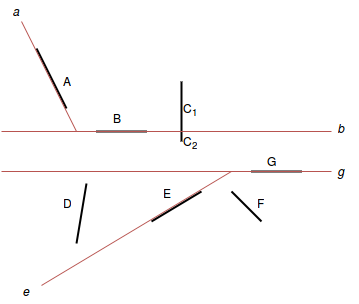
\includegraphics[width=0.9\linewidth]{img/bsp12.png}
  \caption{Taso neljän jaon jälkeen}
  \label{bsp12}
 \end{subfigure}
 \caption{Tason jakaminen}
 \vspace{-0.5cm}
 \label{bsp1}
\end{figure}


BSP-puun kokoon ja muotoon vaikuttaa suuresti avaruuden jakavan monikulmion valinta. Pahimmassa tapauksessa kaikki monikulmio $\Gamma\backslash\{\gamma_k\}$ jäävät monikulmion $\gamma_k$ positiiviselle tai negatiiviselle puolelle jokaisella jaolla $k$. Tällöin puusta muodostuu pikemminkin ketjun muotoinen. Sama monikulmio voi myös kuulua moneen BSP-puun alipuuhun, jos jonkun ylemmällä tasolla avaruuden jakavan monikulmion $\gamma_k$ muodostama jakolinja leikkaa tätä monikulmiota. \citep[.]{samet} Toinen lähestymistapa jakolinjalla oleviin monikulmioihin on halkaista ne kahtia. Tämäkin tapa on epäedullinen, sillä se lisää maisemassa olevien monikulmioiden määrää. \citep[.]{ranta}\\ %Kun otetaan huomioon nämä rajoitteet, ei BSP-puun koolle voida antaa tarkkaa ylärajaa \citep{hughes}.\\

BSP-puuta rakennettaessa tavoitteena on muodostaa mahdollisimman tasapainoinen binääripuu valitsemalla jokaisella jakokerralla jakajaksi sellainen monikulmio $\gamma_k$, jonka positiivisella ja negatiivisella puolella on likimain yhtä paljon monikulmioita, eli $\abs{\Gamma_{k,+}} \approx \abs{\Gamma_{k,-}}$. Tällöin  $n$:n monikulmion joukousta muodostetun BSP-puun syvyys olisi $O(\log n)$, mikäli rekursiivista jakoa jatketaan kunnes jokainen monikulmio on omassa lehdessään. Koska puun solmuja syntyy lisää, kun jakolinjan leikkaavat monikulmiot jaetaan kahtia, tai jakolinjalla oleva monikulmio sisällytetään useaan alipuuhun, voidaan puun logaritmista tavoitesyvyyttä pitää vain alarajana. \citep[.]{hughes} $n$ monikulmiota sisältävästä maisemasta rakennetun BSP-puun syvyys on siis $\Omega(\log n)$.\\

\begin{figure}
 \centering
 \begin{tikzpicture}[level/.style={sibling distance = 60mm/#1}]
  \node[circle,draw] (z){$G$}
    child {node [circle,draw] (a) {$E$}
     child {node [circle,draw] (b) {$D$}}
     child {node [circle,draw] (c) {$F$}}
    }
    child {node [circle,draw] (d) {$B$}
     child {node [circle,draw] (e) {$C_2$}}
     child {node [circle,draw] (f) {$A$}
      child[missing] {node {}}
      child {node [circle,draw] (g) {$C_1$}}}
    };
 \end{tikzpicture}
 \caption{Tasosta muodostettu BSP-puu}
 %\vspace{-0.5cm}
 \label{bsp2}
\end{figure}


BSP-puu voidaan rakentaa ennen hahmontamista esiprosessointivaiheessa. Hahmontamisvaiheessa sitä voidaan käyttää vähentämään säde-monikulmio leikkaustestien määrää. Kamerasta ammuttua sädettä verrataan ensin BSP-puun juurena toimivaan monikulmioon. Jos säde leikkaa monikulmion $\gamma_k$ muodostaman avaruuden jakavan tason, säde voi osua johonkin monikulmioon molemmissa joukoissa ${\Gamma_{k,+}}$ ja ${\Gamma_{k,-}}$, eli joudutaan tarkastelemaan molempia alipuita. Jos säde ei leikkaa jakotasoa, siirrytään tarkastelemaan vain toista alipuuta. Säteen $\vec{R}=O+t\vec{D}$ osumista tasoon $T$ voidaan testata laskemalla etäisyys $t=\dfrac{-\vec{n}\cdot(O-Q_0)}{\vec{n}\cdot\vec{D}}$, missä $\vec{n}$ on tason $T$ normaalivektori ja $Q_0$ on jokin tason $T$ piste. Säde $\vec{R}$ osuu tasoon $T$ jos sijoittamalla $t$ säteen yhtälöön, on piste $Q = O+t\vec{D}$ tasossa $T$. Tämä pitää paikkansa jos $(Q-Q_0)\cdot\vec{n} = 0$. \citep[.]{hughes} Toistamalla säteiden ja avaruuden jakavien tasojen leikkauksia rekursiivisesti, päädytään lopulta BSP-puun juureen ja voidaan testata, osuuko säde monikulmioihin. \citep[.]{ranta}\\
%polygonien lisääminen kesken renderöinnin työlästä

\subsubsection{kd-puu}

BSP-puun erikoistapaus on \emph{kd-puu}, eli k-ulotteinen puu (engl. \emph{k-dimensional tree}). 
%mites ku tässä virke alkaa pienellä?
kd-puussa avaruuden jakavaa tasoa ei valita jakavan monikulmion muodostaman sivun mukaan, vaan jaot tehdään siten, että jakotaso on kohtisuorassa  jotakin koordinaattiakselia vasten. Yleisin tapa muodostaa kd-puu kolmiulotteisen maiseman monikulmioista on valita jakotaso vuorotellen maailmakoordinaatiston $x$-, $y$- ja $z$-akseleiden vastaiseksi. kd-puun jokaiseen solmuun tallennetaan  
% tieto jakosuunnasta eli minkä akselin vastaisesti avaruusjako on tehty. 
jakavan monikulmion sijaan jakava taso. Tällöin monikulmioiden jakaminen solmun lapsiin onnistuu helposti vertaamalla niiden sijaintia jakotasoon. Esimerkiksi jos avaruuden jakava taso valitaan kohtisuoraksi $x$-akselia vasten, tallennetaan solmun vasempaan lapseen monikulmiot, joiden sijainnin $x$-koordinaatin arvo on pienempi kuin jakotason. Oikeaan lapseen taas tallennetaan monikulmiot, jotka ovat jakotason positiivisella puolella $x$-akselin suhteen. \citep[.]{samet} Avaruutta jaetaan rekursiivisesti osiin kunnes lehtisolmuissa on jokin ennaltamäärätty määrä monikulmioita. kd-puu muodostetaan vastaavalla algoritmilla kuin BSP-puun rakentamista kuvaava algoritmi \ref{algo_bsp}.\\

Yleisen BSP-puun tapaan myös kd-puuta rakennettaessa avaruuden jakavien tasojen valinta vaikuttaa siihen, kuinka tehokkaasti puuta voidaan hyödyntää hahmontamisessa. Jakotaso voidaan valita aina jakamalla avaruuden osa tasan kahtia, jolloin samalla syvyydellä puussa olevat solmut vastaavat saman kokoista laatikkoa. Tämä tapa ei takaa sitä, että jakotason molemmille puolille jäisi saman verran monikulmioita, joten puusta ei tule tasapainoista. Hahmontamisen kannalta parempi tapa on käyttää esiprosessointivaiheessa enemmän laskenta-aikaa ja valita jakotaso siten, että sen molemmille puolillä jää likimain yhtä paljon monikulmioita. Sellaiset monikulmiot, jotka leikkaavat avaruuden jakavaa tasoa, täytyy sisällyttää puuhun useaan solmuun tai jakaa ne pienempiin osiin. \citep[.]{havran}\\

\begin{figure}
 \centering 
 \includegraphics[width=0.5\textwidth]{img/bsp3.png}
 %\vspace{0.4cm}
 \caption{Kuvan \ref{bsp11} taso jaettuna kuusi kertaa}
 \vspace{-0.5cm} 
 \label{bsp3}
\end{figure}

Eräs mahdollinen tapa jakaa taso osiin koordinaattiakselien suuntaisesti on esitetty kuvassa \ref{bsp3}, jossa tarkastellaan kuvan \ref{bsp11} tapaan monikulmiot $\Gamma=\{A,B,C,D,E,F,G\}$ sisältävää kaksiulotteista tasoa. Ensin taso jaetaan puoliksi $x$-akselin vastaisella suoralla $q$. Jaon positiiviselle puolelle jäävät monikulmiot $\Gamma_{q,+} = \{C,G,E,F\}$. Kun jaetaan suoran $q$ positiivinen puoli $y$ akselin vastaisella jaolla $r$ ja edelleen $x$ akselin vastaisilla jakosuorilla $s$ ja $t$, on monikulmiot $C$, $G$, $E$ ja $F$ saatu omiin solmuihinsa. Vastaava jako suoritetaan suoran $q$ negatiivisella puolella oleville monikulmioille $\Gamma_{q,-} = \{A,B,C\}$ jakosuorilla $u$ ja $v$, jolloin tason monikulmioista saadaan muodostettua kuvan \ref{bsp4} mukainen kd-puu.\\ 

Muodostamalla esiprosessointivaiheessa maiseman monikulmioista BSP-puun sijaan kd-puu voidaan nopeuttaa säteiden ja avaruuden osien yhteentörmäystestejä. Koska kd-puussa avaruuden jakavat tasot ovat kohtisuorassa koordinaattiakselia $a$ vasten, $a\,\epsilon\,(x, y, z)$, ja jakosuunta on joka solmussa tiedossa, voidaan jakotaso esittää vain yhdellä arvolla $a_p$. Tällöin säteen ja jakotason yhteentörmäyksen testaaminen on noin kolme kertaa nopeampaa kuin satunnaisesti suunnatulle tasolle $ax + by + cz + d = 0$. \citep[.]{havran}\\

\begin{figure}
 \centering
 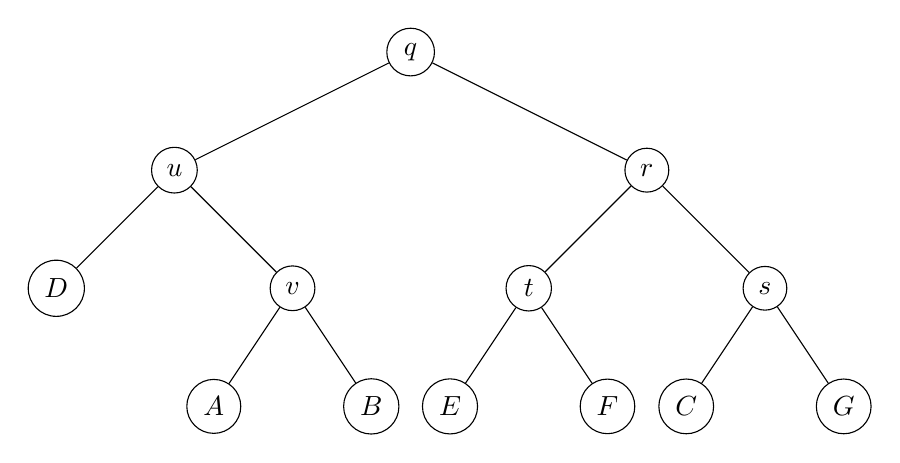
\begin{tikzpicture}[level/.style={sibling distance = 60mm/#1}]
  \node[circle,draw] (z){$q$}
   child {node [circle,draw] (a) {$u$}
    child {node [circle,draw] (b) {$D$}}
    child {node [circle,draw] (c) {$v$}
     child {node [circle,draw] (d) {$A$}}
     child {node [circle,draw] (e) {$B$}}
    }
   }
   child {node [circle,draw] (f) {$r$}
    child {node [circle,draw] (g) {$t$}
     child {node [circle,draw] (h) {$E$}}
     child {node [circle,draw] (i) {$F$}}
    }
    child {node [circle,draw] (j) {$s$}
     child {node [circle,draw] (k) {$C$}}
     child {node [circle,draw] (l) {$G$}}
    }
  };
 \end{tikzpicture}
 \caption{Tasosta muodostettu kd-puu}
 \label{bsp4}
\end{figure}


Muita BSP-puun erikoistapauksia ovat \emph{quad}- ja \emph{oct-puut}. Quad-puuta muodostettaessa avaruuden osa jaetaan aina neljään yhtä suureen kuutioon kunnes jokin pysähtymisehto saavutetaan. Oct-puun tapauksessa kuutioiden määrä on kahdeksan \citep[.]{samet}. Lukuunottamatta ennaltamäärättyä avaruusjakojen määrää quad- ja oct-puut ovat kuten yllä määritellyt kd-puut.

\subsection{Rajaavien tilojen hierarkia}

BSP-puuta objektilähtöisempi tapa jakaa kolmiulotteista avaruutta osiin on määrittää jokaiselle objektille \emph{rajaava tila} (engl. \emph{bounding volume}). Objektin $O$ rajaava tila on jokin yksinkertainen kolmiulotteinen muoto $V$, jolle $O \cap V \equiv O$ \citep{havran}. Useimmiten rajaavan tilan muodoksi valitaan pallo tai koordinaattiakseleiden suuntainen laatikko, sillä säteen osumista niihin on helppo testata.\footnote{Säteen osumatesti kummankin muodon kanssa vaatii noin kymmenen laskutoimitusta \citep{goldsmith}.} Rajaavat tilat tulisi valita siten, että ne rajaavat objekteja tarkasti, jättämättä liikaa tyhjää tilaa itsensä ja objektin väliin. \citep{hughes} \\

\emph{Rajaavien tilojen hierarkia}, eli \emph{BVH} (engl. \emph{Bounding Volume Hierarchy}) on puu, jonka juurena on koko maiseman tilavuus ja solmuissa pienempiä, yhden tai useamman objektin rajaavia tiloja. Puun solmuihin on tallennettu tieto rajaavan tilan muodosta, koosta ja sijainnista, sekä osoittimet lapsisolmuihin. Lehtisolmut ovat pienimpiä rajaavia tiloja, jotka sisältävät yhden objektin tai osan siitä. BVH voidaan muodostaa rakentamalla ensin maisemasta BSP-puu ja sen jälkeen määrittää ympäröiviä tiloja objekteille rekursiivisesti lehtisolmuista ylöspäin. \citep{hughes} Toinen tapa on käydä esiprosessointivaiheessa läpi kaikkien objektien monikulmioiden kärjet ja ottaa talteen maksimi- ja minimiarvot $x_{max}$, $x_{min}$, $y_{max}$, $y_{min}$, $z_{max}$ ja $z_{min}$. Näiden arvojen avulla voidaan muodostaa rajaava tila, jonka sisään kaikki objektin monikulmiot jäävät. \citep[.]{janke} Algoritmissa \ref{algo_bvh} on esitetty eräs tapa alustaa BVH \citep{thrane}.\\

\begin{algorithm}[t]
\small
\KwIn{\\\texttt{monikulmiot}: monikulmiojoukko, josta alipuut rakennetaan}
%\texttt{Polygon monikulmiot[$\,$]}:\tab monikulmiojoukko, josta alipuut rakennetaan}
\KwOut{\\\texttt{BVH\_Node}: BVH:n sisäsolmu}
\BlankLine
\nonl \texttt{RAKENNA\_BVH(monikulmiot):\\}
 \uIf{\textnormal{\texttt{monikulmiot} sisältää vain yhteen objektiin kuuluvia monikulmioita, tai ennalta määrätyn vähimmäismäärän monikulmoita}}{
  \KwRet lehtisolmu, joka sisältää \texttt{monikulmiot}
 }\Else{
  Selvitä taso joka jakaa objektit kahteen, likimain yhtä suureen osaan\\
  \texttt{BVH\_Node solmu}\\
  \texttt{solmu.vasen\_lapsi} $\gets$ \texttt{RAKENNA\_BVH}(monikulmiot jaon vasemmalla puolella)\\  
  \texttt{solmu.oikea\_lapsi} $\gets$ \texttt{RAKENNA\_BVH}(monikulmiot jaon oikealla puolella)\\
  \texttt{solmu.rajaava\_tila} $\gets$ pienin rajaava tila, joka sisältää kaikki \texttt{monikulmiot}\\
  \KwRet \texttt{solmu}} 

\caption{\texttt{RAKENNA\_BVH \citep{thrane}}}\label{algo_bvh}
\end{algorithm}




BVH:n hyödyntäminen hahmontamisessa säteenseurantatekniikalla on yksinkertaista. Kamerasta ammuttavien säteiden osumia testataan ensin BVH:n juureen, minkä jälkeen siirrytään rekursiivisesti molempiin lapsisolmuihin aina kun säde osuu solmuun. Jos käytössä on koordinaattiakselien suuntaiset laatikot, osuu säde $\vec{R}=O+t\vec{D}$ laatikkoon kun se leikkaa laatikon kaksi sivua. Säteen ja tason osumatestiä on kuvailtu luvussa 3.1. Vertailemalla säteen $\vec{R}$ leikkauspisteitä rajaavan tilan sivujen kanssa saadaan etäisyydelle $t$ välit $[t_{x_0}, t_{x_1}]$, $[t_{y_0}, t_{y_1}]$ ja $[t_{z_0}, t_{z_1}]$, joissa alarajat ovat säteen ensimmäisiä ja ylärajat sen toisia leikkauspisteitä laatikon kanssa. Jos jokin arvo $t$ kuuluu kaikkiin näihin väleihin, lävistää säde $\vec{R}$ laatikon, ja siten siirrytään tarkastelemaan joko laatikon sisällä olevia rajaavia tiloja tai sen sisältämiä monikulmioita. \citep[.]{janke}\\

Kuten BSP- ja kd-puun tapauksissa, myös BVH:n tuoma etu hahmontamisessa riippuu siitä, miten hyvin jako rajaaviin tiloihin onnistuu. Kuvassa \ref{bvh1} havainnollistetaan rajaavan tilan valinnan merkitystä. Kuvassa on pisteistä kaksiulotteisessa tasossa ja kaksi vaihtoehtoa niitä rajaavaksi tilaksi. Koordinaattiakseleiden suuntainen laatikko (a) ei ole tässä tapauksessa optimaalinen, vaan jättää pisteiden ja laatikoiden väliin liikaa tyhjää tilaa. Tällöin monet laatikon lävistävät säteet eivät osu itse pisteisiin. Tiiviimpi laatikko on esitetty vieressä (b).\\

\begin{figure}
 \centering 
 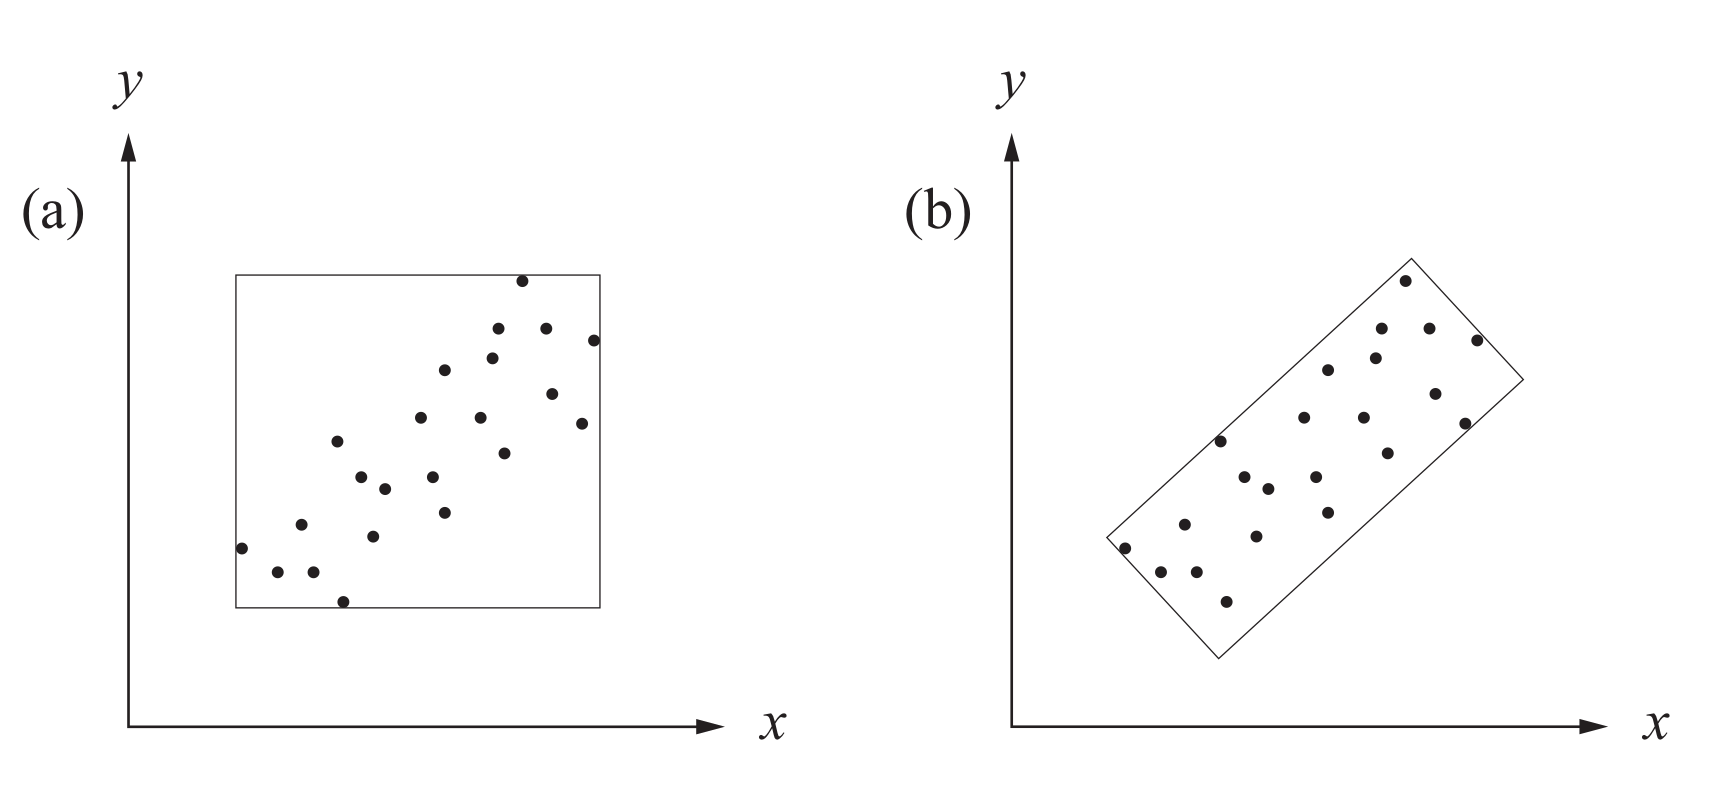
\includegraphics[width=0.8\textwidth]{img/bvh1.png}
 \vspace{0.4cm}
 \caption{Kaksi vaihtoehtoa pistejoukon rajaavaksi tilaksi \citep{lengyel}}%s212
 \vspace{-0.5cm} 
 \label{bvh1}
\end{figure}

Säteen $\vec{R}=O+t\vec{D}$ ja pallon $S$ leikkausta voidaan tarkastella määrittämällä ensin vektori $\vec{a} = C - O$, missä $C$ on pallon $S$ keskipiste. Tällöin saadaan suorakulmainen kolmio, jossa $\vec{a}$ on hypotenuusa ja $\dfrac{\vec{a}\cdot\vec{v}}{\abs{\vec{v}}}$ on kateetti. Laskemalla Pythagoraan lauseella toisen kateetin pituus $d = \sqrt{\vec{a}^2 - (\dfrac{\vec{a}\cdot\vec{v}}{\abs{\vec{v}}})^2}$ saadaan selville mikä on pienin säteen ja pallon keskipisteen välinen etäisyys. Jos $\abs{d} < r$, missä $r$ on pallon $S$ säde, lävistää säde $R$ pallon ja voi osua sen sisältämiin monikulmioihin. \citep[.]{janke}    


\newpage
\section{Avaruusjakopuiden vertailua}

Tässä luvussa vertaillaan luvussa 3 esiteltyjä tietorakenteita ja selvitetään, mitä eroja niissä on säteenseurannan nopeuttamisen kannalta. Lisäksi selvitetään mitä ongelmia tietorakenteiden alustamiseen liittyy, ja miten onglemat voidaan selvittää. Vertailussa keskitytään pääasiassa binääriseen avaruusjakoon kd-puun avulla ja objektien ryhmittelyyn BVH:n avulla. Yleisen BSP-puun sijaan tarkastellaan kd-puuta sen yksinkertaisuuden ja sitä käsittelevän tutkimuksen määrän vuoksi.\footnote{Myös yleisen BSP-puun käyttö säteenseurannassa on tuottanut hyviä tuloksia. \citep[ks. esim.][]{ranta}} 

\subsection{Tietorakenteiden alustaminen}

Rakennettaessa kd-puuta on otettava kantaa, mitä tehdään monikulmioille, jotka ulottuvat avaruuden jakavan tason molemmille puolille. Sekä monikulmion jakaminen osiin, että sen sisällyttäminen useaan solmuun kasvattavat kd-puuta turhaan. kd-puusta saatava hyöty on suurin silloin, kun avaruusjakoja on tehty mahdollisimman paljon ja lehtisolmuissa on mahdollisimman vähän monikulmioita. Tällöin todennäköisyys sille, että monikulmioita jää jakotasojen molemmin puolin on suuri ja tietorakenteen vaatima tallennustila kasvaa erittäin suureksi. \citep[.]{wald04} \\

BVH:ta muodostettaessa ei synny samankaltaista ongelmaa kuin kd-puiden kanssa, sillä monikulmio voi kuulua vain yhteen objektiin ja objektin rajaava tila sisältää kaikki sen monikulmiot. Myös BVH-puu kannattaa muodostaa syväksi. Jos BVH sisältäisi vain koko maiseman kattavan juuren ja sen lapsina olisi kaikkien objektien rajaavat tilat, ei tietorakenteen tuoma hyöty olisi paras mahdollinen. Puuhun kannattaa siis sijoittaa useita rajaavia tiloja, jotka sisältävät useita objekteja. Objektijoukon jakaminen kahtia BVH:n jokaisella tasolla  näyttäisi olevan hyvä valinta. \citep[.]{goldsmith} \\

Kuten aikaisemmin mainittu, avaruusjakorakenteen tuoma hyöty riippuu siitä, miten hyvin avaruuden ositus on onnistunut. Sekä kd-puun, että BVH:n alustamisessa voidaan hyödyntää samankaltaista hintafunktiota, jolla voidaan minimoida puun läpikäymisen viemä aika. Hintafunktiota voidaan kuvata seuraavasti: olkoon alipuussa $N$ monikulmiota, jotka peittävät alueen $V$. Tämä alipuu jaetaan osiin $L$ ja $R$, joissa on $N_L$ ja $N_R$ monikulmiota, jotka peittävät alueen $V_L$ ja $V_R$. Tällöin alipuun läpikäymisen hinta on\\

\begin{centering} 
$Hinta(V\to\{L,R\}) = K_T + K_I(\dfrac{A(V_L)}{A(V)}N_L + \dfrac{A(V_R)}{A(V)}N_R)$,\\
\vspace{0.2cm}
\end{centering}
missä $A(V_i)$ on alueen $V_i$ pinta-ala, ja arvot $K_T$ ja $K_I$ ovat joitakin puun läpikäynnistä ja säde-monikulmio-yhteentörmäystesteistä johtuvia vakioita. Minimoimalla tämä funktio puun alustuksen joka vaiheessa, saadaan muodostettua tehokas avaruuden jako. \citep[.]{wald07}\\

Edellä mainittua, hintafunktiota käyttävää tekniikkaa kutsutaan \emph{pinta-ala heuristiikaksi} (engl. \emph{Surface Area Heuristics, SAH}) ja sillä saadaan muodostettua hyvä avaruuden ositus sekä kd-puulle, että BVH:lle. Ingo Waldin tekemässä tutkimuksessa BVH:n muodostaminen onnistui kuitenkin jopa 10 kertaa nopeammin. Tämä johtuu muun muassa kd-puun alustamisessa esiintyvistä, jakotason leikkaavista monikulmioista. \citep[.]{wald07}  

%BVH:n muodostaminen maisemasta vie vain n. 30\% enemmän tilaa. golds

%BVH:ssa nodeja on O(2n-1) wald

\subsection{Tietorakenteiden hyödyntäminen säteenseurannassa}

Avaruusjakorakenteiden hyödyntäminen säteenseurannassa on hyvin samankaltaista riippumatta siitä, millä periaatteella tietorakenne on muodostettu. Algoritmissa \ref{algo_isect} on kuvattu hyvin yksinkertainen pseudokoodi, jolla voidaan testata säteen osumista avaruusjakopuuna kuvattuun maisemaan.\\ 

\begin{algorithm}[htp]
\small
\KwIn{\\$\vec{R}$: kamerasta ammuttu säde\\
\texttt{Solmu s}: jonkin avaruusjakopuun solmu}
\KwOut{\\Kolmio, johon säde $\vec{R}$ osui}
\BlankLine
\nonl \texttt{SÄDE\_PUU\_YHTEENTÖRMÄYS($\vec{R}$, s):\\}
 \uIf{\textnormal{$\vec{R}$ osui solmun \texttt{s} kuvaamaan avaruuden osaan}}{
   \If{\textnormal{\texttt{s} on lehtisolmu}}{
    \KwRet \tiny SÄDE\_MONIKULMIO\_YHTEENTÖRMÄYS \small ($\vec{R}$, \texttt{s.monikulmiot})
   }
   \texttt{SÄDE\_PUU\_YHTEENTÖRMÄYS($\vec{R}$, s.oikea\_lapsi)}\\
   \texttt{SÄDE\_PUU\_YHTEENTÖRMÄYS($\vec{R}$, s.vasen\_lapsi)}
  }\Else{
   \KwRet \texttt{NULL}
} 

\caption{\texttt{SÄDE\_PUU\_YHTEENTÖRMÄYS}}\label{algo_isect}
\end{algorithm}



%Vlastimil Havran   \citep[]{havran}\\

Niels Thrane ja Lars Ole Simonsen vertailivat pro gradu -työssään eri avaruusjakorakenteita grafiikkaprosessoreilla suoritetussa säteenseurannassa. Koska säteenseurannassa jokainen säde on riippumaton muista säteistä, voidaan säteenseuranta-algoritmi suorittaa helposti rinnakkain, mikä onnistuu grafiikkaprosessoreilta erittäin nopeasti. Yllättäen Thranen ja Simonsenin vertailussa BVH:n käytöllä saatiin yhdeksänkertainen nopeutus kd-puuhun verrattuna. \citep[.]{thrane}\\  

Yksiselitteisesti ei voida sanoa, mikä avaruusjakoon perustuvista tietorakenteista soveltuisi parhaiten säteenseurannan nopeuttamiseen. Asymptoottisesti avaruusjakopuiden käyttö säteenseurassa vähentää tarvittavien yhteentörmäystestien määrää luokasta $O(n)$ luokkaan $O(\log n)$, riippumatta käytetystä tietorakenteesta. Tulokset voivat vaihdella käytännössä eri maisemien, implementaatioiden, laitteistojen ja sovelluksien välillä. \citep[.]{wald04}  


%Säteen ja lähimmän monikulmion leikkauspisteen etsintä voidaan lopettaa heti ensimmäinen leikkaus, jos monikulmiot on jaettu esiprosessointivaiheessa kasvavaan järjestykseen etäisyyden kamerasta kannalta \citep{wald04}

%BVH:n topologia voidaan pitää muuttumattomana liikkuvassa maisemassa ja vain siirtää rajaavia tiloja objektien liikkuessa. Täten sen päivittäminen maiseman liikkuessa on helpompaa kuin tilallisten rakenteiden, kuten BSP-puun ja kd-puun. \citep[.]{wald}

%Thrane väittää gradussaan, että BVH on n. 9 kertaa tehokkaampi gpu-hahmontamisessa. \citep{thrane}
%Koska säteenseurannassa jokainen säde on riippumato muista, voidaan säteenseuranta-algoritmi suorittaa helposti rinnakkain. 
%GPUt ovat erittäin nopeita laskemaan grafiikkaan ja kolmioihin liittyviä laskutoimituksia rinnakkain 


\newpage
\section{Yhteenveto}
%hughes sivulla 1102 on hyvä yhteenveto
%Sädepakettien käyttö \citep{wald}
%Portaalit
%mailboxing thrane

\clearpage
\bibliographystyle{apalike} %apalike-finnish
\bibliography{bibliography}
\clearpage
\listofalgorithms
%\listoffigures
\end{document}
